\documentclass[review]{elsarticle}

\usepackage{xr} %% For cross-referencing supl figures
\externaldocument[S-]{Supplementary}

\usepackage{lineno,hyperref}
\usepackage[utf8]{inputenc}
\usepackage{graphicx}
\usepackage{amsfonts}
\usepackage{mathtools}

%% for the annex figure
\usepackage{tikz}
\usetikzlibrary{shapes,arrows,chains,calc}
% Set up a few colours for tikz figure
\colorlet{lcfree}{green}
\colorlet{lcnorm}{blue}
\colorlet{lccong}{red}

\usepackage{hhline}
\usepackage{booktabs}
%\usepackage[textsize=scriptsize]{todonotes}
\usepackage[textsize=scriptsize, disable]{todonotes}  %% to turn off notes
\usepackage{eurosym}
\usepackage{longtable}

\usepackage{enumitem}

% For track-changes
%\usepackage[draft]{changes}
\usepackage[final]{changes} %% to turn off changes
\definechangesauthor[color = red]{JM}
\definechangesauthor[color = blue]{PD}
\definechangesauthor[color = green!40!black]{JJ}
\definechangesauthor[color = purple]{CM}

\modulolinenumbers[1]

\journal{Ecological Modelling}

%% Harvard
\bibliographystyle{model2-names.bst}\biboptions{authoryear}
%%%%%%%%%%%%%%%%%%%%%%%
%% correct equation line numbering

\let\oldequation\equation
\let\oldendequation\endequation
\renewenvironment{equation}
 {\linenomathNonumbers\oldequation}
 {\oldendequation\endlinenomath}


%%%%%%%%%%%%%%%%%%%%%%



\begin{document}

\begin{frontmatter}
\title{\emph{MixFishSim}: highly resolved spatiotemporal simulations for
	exploring mixed fishery dynamics}

%% Group authors per affiliation:
\author[1,2]{Paul J. Dolder\corref{c}}
\cortext[c]{Corresponding author}
\ead{paul.dolder@gmit.ie}

\author[1]{Cóilín Minto}
\author[3]{Jean-Marc Guarini}
\author[4]{Jan Jaap Poos}

\address[1]{Galway-Mayo Institute of Technology (GMIT), Dublin Road, Galway,
	Ireland} 
\address[2]{Centre for Environment, Fisheries and Aquaculture Science (Cefas),
	Pakefield Road, Lowestoft, UK}
\address[3]{\replaced[id=JM]{Sorbonne Université, Faculty of
		Sciences}{Université Pierre et Marie Curie}, 4 Place Jussieu,
	75005 Paris, France}
\address[4]{Wageningen Marine Research, Haringkade 1 1976 CP IJmuiden,
	Netherlands}

\begin{abstract}

\replaced[id = JJ]{Most fisheries}{Fishing} exploit\deleted[id=JJ]{s} a variety 
of spatially and temporally heterogeneous fish populations using
species-unselective gear that can result in unintended, unwanted catch of low
quota or protected species. Reducing these unwanted catches is crucial for
biological and economic sustainability of `mixed fisheries' and implementation
of an ecosystem approach to fishing. \\

\replaced[id = PD]{If fisheries are to avoid unwanted catch,}{To implement
	effective spatial measures to reduce discards} a good understanding of
spatiotemporal fishery dynamics is required. However, traditional scientific
advice is limited by a lack of highly resolved knowledge of population
distributions, population movement and how fishers interact with different fish
populations. This reflects the fact that data on fish location at high temporal
and spatial resolutions is expensive and difficult to collect. Proxies inferred
from either scientific surveys or commercial catch data are often used to model
distributions, usually with sparse data at limited spatial and temporal
resolution. \\ 

To understand how data resolution impacts inference on mixed fisheries
interactions, we developed a highly resolved spatiotemporal simulation model
incorporating: i) delay-difference population dynamics, ii) population movement
using Gaussian Random Fields to simulate patchy, heterogeneously distributed
populations, and iii) fishery dynamics for multiple fleet characteristics based
on species targeting under an explore-exploit strategy via a mix of correlated
random walk movement (for exploration) and learned behaviour (for exploitation)
phases of the fisheries.  \\ 

We simulated 50 years of fishing and used the results from the fisheries catch
to draw inference on the underlying community structures. We compared this
inference to a simulated fixed-site sampling design commonly used for fisheries
monitoring purposes and the true underlying community structure. We i) used
the results to establish the potential and limitations of fishery-dependent
data in providing a robust picture of spatiotemporal distributions; and ii)
simulated an area closure based on areas defined from the different data sources
at a range of temporal and spatial resolutions to assess their effectiveness
on reducing catches of a fish population. \\

Our framework allows users to explore the assumptions in modelling
observational data and evaluate the underlying dynamics of such approaches at a
fine spatial and temporal scale. We conclude from our simulations that
commercial data, while containing bias, provide a useful tool for managing
catches in mixed fisheries if applied at the correct spatiotemporal scale. \\

\end{abstract}

\begin{keyword}
Some\sep keywords \sep here. Max 6 
\MSC[2010] 00-01\sep  99-00
\end{keyword}

\end{frontmatter}

\linenumbers

\section{Introduction}

Fishers exploit a variety of fish populations that are heterogeneously
distributed in space and time, with varying knowledge of species
distributions\deleted[id=JJ]{ and using species non-selective fishing gear}.
\added[id=PD]{In doing so} fisheries \deleted[id=PD]{that}catch an assemblage
of species \added[id=PD]{and}\deleted{, known as mixed fisheries}
\replaced[id=JJ]{may}{, when managed by single-species quotas can end up}
discard\deleted[id=JJ]{ing} over-quota catch \added[id=JJ]{when managed by
	single species quotas and fishers exhaust one or more quota. This may}
lead to overexploitation of fish populations \added[id=JJ]{\citep{Ulrich2011a,
		Batsleer2015}}.  \added[id=JJ]{Discarding of fish in
	excess of quota limits the ability to maintain fishing mortality within
	sustainable limits \citep{Alverson1994, Crowder1998, Rijnsdorp2007}}
\deleted[id=PD]{; reducing discarding is crucial}and the ability to manage for
the biological and economic sustainability of fisheries\deleted[id=JJ]{ and
	implementation of an ecosystem approach to fisheries}. As such, there
is increasing interest in technical solutions such as gear and spatial closures
as measures to \replaced[id=PD]{reduce unwanted catch}{avoiding
	discard\added[id=JJ]{ing of fish}} \citep{Kennelly2002, Catchpole2008,
	Bellido2011, Cosgrove2019}.  \\

\replaced[id=PD]{Adaptive spatial management strategies have}{Use of spatial
	management as a tools} been proposed as a way of reducing discards
\added[id=PD]{\citep{Holmes2011, Little2014, Dunn2014a}}.  \deleted[id=PD]{its}
Implementation of avoidance measures is, however, restricted by lack of
knowledge of fish and fishery spatiotemporal dynamics and understanding of the
scale at which processes become important for management. Understanding the
correct scale for spatial measures is crucial for implementing solutions at a
resolution that ensures effective management \citep{Dunn2016} while minimising
economic impact.  For example, the problem can be to identify a scale that
promotes species avoidance for vulnerable or low quota species while allowing
continuance of sustainable fisheries for available quota species.\\

\replaced[id=PD]{Identifying}{Ensuring measures are implemented at} appropriate
spatial scales for fisheries closures has been a challenge in the past but
identified as crucial to its success \citep{Costello2010, Dunn2016}. Further,
poorly sited closures have led to ineffectual measures with unintended
consequences. For example, increased benthic impact on previously unexploited
areas was observed from the cod closure in the North Sea with a lack of
observed intended effect in reducing cod exploitation
\citep{Rijnsdorp2001,Dinmore2003}). \replaced[id=PD]{M}{Since then m}ore
refined spatiotemporal information has \added[id=PD]{since} become available
through the combination of logbook and Vessel Monitoring System (VMS) data
\citep{Lee2010, Bastardie2010, Gerritsen2012, Mateo2016} and more real-time
spatial management has been possible \citep[e.g.][]{Holmes2011}.  Such
information is, however, derived from an inherently biased sampling programme,
targeted fishing, where fishers establish favoured fishing grounds through an
explore-exploit strategy \citep{Bailey2018} where they search for areas with
high catches and then use experience to return to areas where they've
experienced high catch in the past.  \deleted[id=PD]{ Further, fishers
	generally only recorded landings (not catch) on a daily
	basis\todo{\added[id=JJ]{Its not clear what the problem is: landings
			collected on daily basis or landings recorded rather
			than catch}}.  This leads to questions about the
	validity of inference that can be drawn from landings data assigned to
	VMS activity pings.}\todo{\added[id=JJ]{This comes as a surprise: I
		thought this was going to be about
		discards}\added[id=PD]{Agree, have removed this to avoid
		confusion}}\\ 

\replaced[id=PD]{In order to understand the effect of spatiotemporal
	aggregation of data we ask two fundamental questions regarding
	inference derived from observational data:}{ and use the
	results}\deleted[id=PD]{ from the fishing model:}

\begin{enumerate}
	\item How does sampling-derived fisheries data reflects the underlying
		community structure? 	
	\item How does data aggregation and source impact on spatial fisheries
	management measures?
\end{enumerate}
	
To answer these questions we i) develop a simulation model where population
dynamics are highly-resolved in space and time by use of a Gaussian spatial
process to define suitable habitat\replaced[id=PD]{. Precise locations being}{
	and are} known \added[id=PD]{directly} rather than inferred from
sampling or commercial catch\added[id=PD]{, we can use the population model to
	validate how inference from fisheries-dependent and fisheries
	independent sampling relates to the real community structure in a way
	we could not with real data}. We ii) compare, at different spatial and
temporal aggregations, the 'real population' distributions to samples from
fisheries-dependent and fisheries independent catches to test if these are a
true reflection of the relative density of the populations. We then iii)
simulate a fishery closure to protect a species based on different spatial and
temporal data aggregations. We use these evaluations to draw inference on the
utility of commercial data in supporting management decisions.
\todo{\added[id=JJ]{If the paper has two goals this should be clear from the
		start, but may be better over 2 MSs}\added[id=PD]{I would like
		to keep both parts, but have made clearer in how its set out.
		The closure scenarios form validation of the data aggregation,
		rather than effectiveness of the closures themselves - so its a
		continuation of the same question in my eyes}}\deleted[id=PD]{.
	Further, we extend our analysis to a range of spatial and temporal
	scales to assess the impact of these processes on the success of the
	management measure.}\\

\section{Materials and Methods}

\replaced[id=PD]{A}{We developed and implemented a simulation model with a}
\replaced{simulation model that is modular and discrete-event based was
	developed. This approach enables efficient computation by allowing
	for}{approach, where} \added[id=PD]{sub-}modules \deleted[id=PD]{are}
implemented on time-scales appropriate to capture the characteristic of the
\replaced[id=PD]{different processes}{process modelled} (Figure 1).
\added[id=PD]{The following sub-modules were included to capture the full
	system: 1) Population dynamics, 2) Recruitment dynamics, 3) Population
	movement, 4) fishery dynamics.}\\

\deleted[id=PD]{The fishing model operated on a tow-by-tow basis, while}
\replaced[id=PD]{P}{p}opulation dynamics (fishing and natural mortality which
are instantaneous rates, growth of the population biomass) operate on a daily
time-step\replaced[id=PD]{, while p}{. P}opulation movement occurs on a weekly
time-step\replaced[id=PD]{. R}{, while r}ecruitment \replaced[id=PD]{takes
	place}{occurs} periodically each year for a set time
\replaced[id=PD]{duration}{period (e.g. 3 weeks)} specified for each
population\deleted[id=PD]{.}\added[id=PD]{, while the fishing module operates
	on a tow-by-tow basis (i.e. multiple events a day)}.
\deleted[id=PD]{Here we describe each of the model components; 1) Population
	dynamics, 2) Recruitment dynamics, 3) Population movement dynamics, 4)
	fishery dynamics.}

Population movement is a combination of random (diffusive) movement, governed
by a stochastic process where movement between adjacent cells is described by a
set of probabilities, and directed (advective) movement where at certain times
of year the population moves towards spawning grounds by increasing the
probabilities of moving into the spawning grounds from adjacent cells. We
incorporate characterisation of a number of different fishing
\added[id=PD]{fleet dynamics} exploiting four fish populations with different
spatial and population demographics. The following describes the implementation
of each of the sub-modules.

\subsection{Population dynamics}

The basic population level processes were simulated using a modified two-stage
Deriso-Schnute delay difference model which models the fish populations in
terms of aggregate biomass of recruits and mature components rather than
keeping track of individuals\citep{Deriso1980, Schnute1985, Dichmont2003}.
\added[id=PD]{A daily time-step was chosen to discretise continuous population
	processes on a biologically relevant and computationally tractable
	timescale.} \deleted[id=PD]{Here,}Population biomass growth and
depletion for pre-recruits and\deleted[id=PD]{fish} recruited
\added[id=PD]{fish}\deleted[id=PD]{to the fishery} were modelled separately as
a function of previous recruited biomass, intrinsic population growth and
recruitment functionally linked to the adult population size.  Biomass for each
cell $c$ was incremented each day $d$ as follows (the full parameter list is
detailed in Table \ref{tab: pop_variable}): 
\begin{equation}
	\begin{split}
	B_{c,d+1} = &\\
	& (1 + \rho) B_{c,d} \cdot e^{-Z_{c,d}} - \rho \cdot e^{-Z_{c,d}} \hspace{2.9cm}
	\times \\  
	& (B_{c,d-1} \cdot e^{-Z_{c,d-1}} + Wt_{R-1} \cdot \alpha_{d-1} \cdot
	R_{\tilde{y}(c,y,d-1)})
	\hspace{0.4cm} + \\
	& Wt_{R} \cdot \alpha_{d} \cdot R_{\tilde{y}(c,y,d)} 
	\end{split}
\end{equation}
where $\rho$ is Brody's coefficient, shown to be equal to $e^{-K}$ when $K$ is
the growth rate from a von Bertalanffy logistic growth model
\citep{Schnute1985}. $Wt_{R-1}$ is the average weight of fish prior to
recruitment, while $Wt_{R}$ is the average recruited weight. $\alpha_{d}$
represents the proportion of fish recruited during that day for the year, while
$R_{c,\tilde{y}}$ is the annual recruits in cell $c$ for year $y$. \\

Mortality $Z_{c,d}$ can be decomposed to natural mortality, $M_{c,d}$, and
fishing mortality, $F_{c,d}$, where both $M_{c,d}$ and $F_{c,d}$ are
instantaneous rates with $M_{c,d}$ fixed and $F_{c,d}$ calculated by solving
the Baranov catch equation \citep{Hilborn1992b} for $F_{c,d}$:
\begin{equation}
C_{c,d} = \frac{F_{c,d}}{F_{c,d} + M_{c,d}} * (1 - e^{-(F_{c,d} + M_{c,d})})
\cdot B_{c,d}
\end{equation}
where $C_{c,d}$ is the summed catch from the fishing model across all fleets
and vessels in cell $c$ for the population during the day $d$, and $B_{c,d}$
the daily biomass for the population in the cell. Here, catch and fishing
mortality are the sum of those across all fleets and vessels, where $F_{fl, v,
	c, d, p} = E_{fl, v, c, d} \cdot Q_{fl, p} \cdot D_{c, d, p}$ with
$fl$, $v$ and $p$ the fleet, vessel and population respectively and $E$ and $Q$
fishing effort and catchability of the gear, and $D$ is the density of the
population at the location fished. \todo{\added[id=CM]{[link $F$ to effort and
		catchability - as I think we have F as an emergent property of
		the fleets rather than something we solve for (I could be wrong
		though!) - catch for a vessel is a product of catchability and
		biomass, i.e. C = qB, but this catch is summed to solve for F.
		So its both really]}}\\

\subsection{Recruitment dynamics}

Recruitment is modelled through a function relating the adult biomass to
recruits at time of recruitment. In \emph{MixFishSim}, it can be modelled
either either as a stochastic Beverton-Holt stock-recruit form
\citep{Beverton1957}: 
\begin{equation}
	\begin{split}
	\bar{R}_{c,d} = & \frac{(\alpha \cdot S_{c,d})}{(\beta + S_{c,d})} \\
	     R_{c,d} \sim & \log N[(\log(\bar{R}_{c,d}),\sigma^2)]
	\end{split}
\end{equation}
Where $\alpha$ is the maximum recruitment rate, $\beta$ the spawning stock
biomass (SSB) required to produce half the maximum stock size, $S$ current
stock size and $\sigma^2$ the variability in the recruitment due to stochastic
processes, or a stochastic Ricker form \citep{Ricker1954}:
\begin{equation}
	\begin{split}
	\bar{R}_{c,d} = & B_{c,d} \cdot e^{(\alpha - \beta \cdot B_{c,d})} \\	
   	     R_{c,d} \sim & \log N[(\log(\bar{R}_{c,d}),\log(\sigma^2))]
	\end{split}
\end{equation}
where $\alpha$ is the maximum productivity per spawner and $\beta$ the density
dependent reduction in productivity as the SSB increases. In our example
application the Beverton-Holt form of stock recruit relationship was used for
all populations though either functional form can be chosen.

\subsection{Population movement dynamics}

To simulate \deleted[id=JJ]{how} fish population\deleted[id=JJ]{s might be}
distribut\replaced[id=JJ]{ion}{ed} in space and time\deleted[id=JJ]{, we
	employed} a Gaussian spatial process \added[id=JJ]{was employed} to
model habitat suitability for each of the populations on a 2d grid. JM: MENTION
IN THE INTRODUCTION \\

\deleted[id=PD]{the habitat}We first define\added[id=PD]{d} a Gaussian random
field process\todo{\added[id=JJ]{Not clear how habitat/GRF affect local
		abundances, only have $B_{y,d}$}\added[id=PD]{Have included
		cell reference, $c$ to make spatial link explicit}}, $\{S(c) :
c \in \mathbb{R}^2\}$, \deleted[id=PD]{that is a stochastic process} where
\added[id=PD]{for} any set of cells $c_{1}, \dots, c_{n}$ \deleted[id=PD]{where
	for each $c_{i} \in \mathbb{R}^2$}, the joint distribution of $S =
\{S(c1),\dots S(c_{n})\}$ is multivariate Gaussian with a \textit{Matérn}
\deleted[id=PD]{family of}covariance structure\deleted[id=PD]{s},
\replaced[id=PD]{where}{one where} the correlation strength weakens with
distance\deleted[id=PD]{(i.e. the correlation between $S(x)$ and $S(x')$
	decreases as the distance $u = ||x - x'||$ increases)}.
\added[id=PD]{This enables us to model the spatial autocorrelation observed in
	animal populations where density is more similar in nearby locations
	\citep{Tobler1970, F.Dormann2007}} and we change the parameters to
implement different spatial structures for the populations. \\

\replaced[id=PD]{T}{In the simulation model, t}he habitat for each of the
populations \replaced[id=PD]{was}{is} generated \replaced[id=PD]{with}{through}
the \textit{RFSimulate} function of the \textit{RandomFields} R package
\citep{Schlater2015}, that simulates a Gaussian Random Field process given a
user defined error model and correlation structure. We define a stationary
habitat field and combine with a temporally dynamic thermal tolerance field to
imitate two key drivers of population dynamics. Each population
\replaced[id=PD]{was}{is} initialised at a single location, and subsequently
move\replaced[id=PD]{d}{s} according to a probabilistic
distrib\added[id=PD]{u}tion based on habitat suitability (represented by the
normalised values from the GRFs), temperature and distance
from current cell\replaced[id=PD]{:}{.} 
\begin{equation}
	Pr(J | I) = \frac{e^{-\lambda * d_{IJ}} \cdot
		(Hab_{J,p}^2 \cdot Tol_{J,p,wk})}{\sum\limits_{c=1}^{C}e^{-\lambda * d} \cdot
		(Hab_{c,p}^2 \cdot Tol_{c,p,wk})}
\end{equation}
Where $d_{IJ}$ is the euclidean distance between cell $I$ and cell $J$,
$\lambda$ is a given rate of decay, $Hab_{J,p}^2$ is the squared index of
habitat suitability for cell $J$ and population $p$, with $Tol_{J,p,wk}$ the
temperature tolerance for cell $J$ by population $p$ in week $wk$ (see
below).\\

During pre-defined weeks of the year the habitat suitability is modified with
\added[id=PD]{user-defined} spawning habitat locations\deleted[id=PD]{s},
\replaced[id=PD]{resulting in}{meaning} each population
\replaced[id=PD]{having}{has} concentrated areas where spawning takes place. In
the simulations the populations move\deleted[id=PD]{s} towards
\replaced[id=PD]{these cells}{this} in the weeks prior to spawning, resulting
in directional movement towards the spawning grounds.\todo{\added[id=JM]{What
		does it mean concisely? Areas are assigned?} \added[id=PD]{Yes,
		the areas are pre-defined - I have amended to reflect and tried
		to clarify}} \\ JM: WHAT ABOUT INDIVIDUAL INTERACTIONS:w


\replaced[id=JJ]{An}{, with an} advection-diffusion process\deleted[id=JJ]{to}
control\added[id=JJ]{s}\deleted[id=JJ]{how the} population\deleted[id=JJ]{s}
move\replaced[id=JJ]{ment}{d}, with a time-varying temperature covariate used
to change the interaction between time and suitable habitat on a weekly
time-step\todo{\added[id=JJ]{What have a temperature covariate? Could just use
		time}\added[id=PD]{Was intended as some biological meaning -
		species thermal tolerances load onto the temperature effect -
		so could be different per species}}.  \deleted[id=JJ]{This was
	intended to balance realism in population movement, capturing the main
	directed and random processes, and practicality of modelling the
	population rather than individual fish.} Each population $p$
\replaced[id=PD]{wa}{i}s assigned a thermal tolerance with mean,
$\mu\added[id=PD]{_{p}}$ and variance, $\sigma^2\added[id=PD]{_{p}}$ so that
each cell and population temperature suitability is defined that:
\begin{equation}
	Tol_{c, p\added[id=PD]{, wk}} = \frac{1}{ \sqrt (2\pi \cdot \sigma^2_{p})} \cdot \exp(-
		\frac{(T_{c\added[id=PD]{, wk}} - \mu_{p})^2}{2 \cdot \sigma^2_{p}} )	
\end{equation}
Where $Tol_{c, p, \added[id=PD]{wk}}$ is the tolerance of population $p$ for
cell $c$ \added[id=PD]{in week $wk$}, $T_{c, \added[id=PD]{wk}}$ is the
temperature in the cell \added[id=PD]{given the week} and
$\mu\added[id=PD]{_{p}}$ and $\sigma^2\added[id=PD]{_{p}}$ the mean and
standard deviation of the population temperature tolerance. \\

\added[id=PD]{The final process results in a population structure and movement
	pattern unique to each species, with population movement occurring on a
	weekly basis. The decision to model population movement on a weekly
	timescale was to reflect that fish tend to aggregate in species
	specific locations that have been observed to last around one to two
	weeks \citep{Poos2007}.  Therefore this process approximated the
	demographic shifts in fish populations throughout a year with seasonal
	spawning patterns (e.g.  Figure \ref{S-fig:5}).}

\subsection{Fleet dynamics}

The fleet dynamics can be broadly categorised into three components; fleet
targeting - that determined the fleet catch efficiency and preference towards a
particular species; trip-level decisions, that determined the initial location
to be fished at the beginning of a trip; and within-trip decisions, that
determined movement from one fishing spot to another within a trip. Together,
these elements implemented an explore-exploit type strategy for individual
vessels to maximise their catch from an unknown resource distribution
\cite{Bailey2018}.  The decision to use an individual based model for fishing
vessels was taken because fishers are heterogeneous in their location choice
behaviour due to different objectives, risk preference and targeting preference
\citep{VanPutten2012a}. Therefore in the simulations fleet dynamics are the
productive of individual experiences rather than pre-defined group dynamics. 

\subsubsection{Fleet targeting}

Each fleet of \textit{n} vessels \replaced[id=PD]{was}{is} characterised by
both a general efficiency, $Q_{fl}$, and a population specific efficiency,
${Q_{fl, p}}$.  Thus, the product of these parameters [$Q_{fl} \cdot Q_{fl,
	p}$] affect\replaced[id=PD]{s}{ed} the overall catch rates for the
fleet and the preferential targeting of one population over another. This, in
combination with the parameter choice for the step-function
\added[id=PD]{defined below} (as well as some randomness from the exploratory
fishing process) determine\replaced[id=PD]{d}{s} the preference of fishing
locations for the fleet.  All species prices \replaced[id=PD]{were}{are} kept
the same across fleets \replaced[id=PD]{and seasons}{, though can be made to
	vary seasonally}.  

\subsubsection{Trip-level decisions}

Several studies \citep[e.g.][]{Hutton2004, Tidd2012, Girardin2015} have
confirmed past activity and past catch rates are strong predictors of fishing
location choice. For this reason, the fleet dynamics sub-model
include\replaced[id=PD]{d}{s} a learning component, where a vessel's initial
fishing location in a trip \replaced[id=PD]{wa}{i}s based on selecting from
previously successful fishing locations. This \replaced[id=PD]{wa}{i}s achieved
by \added[id=PD]{calculating an expected revenue based on the catches from
	locations fished} in the preceding trip as well as the same month
periods in previous years and the travel costs from the port to the fishing
grounds, and choosing randomly from the top 75 \% of fishing events
\replaced[id=PD]{as defined by the expected profit, that has a seasonal
	component}{in value}. 

\subsubsection{Within-trip decisions}

Fishing locations within a trip are \added[id=PD]{initially} determined by a
modified random walk process. \added[id=PD]{As the simulation progresses the
	within-trip decision become gradually more influenced by experience
	gained from past fishing locations (as per the initial trip-level
	location choice), moving location choice towards areas of higher
	perceived profit.} A random walk was chosen for the exploratory fishing
process as it is the simplest assumption commonly used in ecology to describe
\added[id=PD]{optimal} animal\deleted[id=PD]{movement which}
search\replaced[id=PD]{ strategy}{ing} for \added[id=PD]{exploiting}
homogeneously distributed prey about which there is uncertain knowledge
\citep{Viswanathan1999}. In a random walk, movement is a stochastic process
through a series of steps\added[id=JJ]{. These steps have a length, and a
	direction} that can either be equal in length or take some other
functional form. The direction of the random walk was also correlated (known as
`persistence') providing some overall \deleted[id=PD]{location of}directional
movement \citep{Codling2008}\deleted[id=PD]{or uncorrelated}. \\

We use a \textit{\replaced[id=JJ]{Lévy flight} {lévy walk}} which is a
particular form of random walk characterised by a heavy-tailed distribution of
step-length\replaced[id=JJ]{. The Lévy flight}{and} has received a lot of
attention in ecological theory in recent years as having shown to have very
similar characteristics as those observed by animals in nature, and being a
near optimum searching strategy for predators pursuing patchily distributed
prey \citep{Viswanathan1999, Bartumeus2005, Sims2008}.  \citet{Bertrand2007}
showed that Peruvian anchovy fishermen have a stochastic search pattern similar
to that observed with a lévy flight. However, it remains a subject of debate
\added[id=PD]{\citep[e.g. see][]{Edwards2011, Reynolds2015}}, with the
contention that search patterns may be more simply characterised as random
walks \citep{Sakiyama2013} with specific patterns related to the
characteristics of the prey field \citep{Sims2012}. \\

For our implementation of a random walk directional change is based on a
negatively correlated circular distribution where a favourable fishing ground
is likely to be ``fished back over" by the vessel returning in the direction it
came from.  The step length (i.e. the distance travelled from the current to
the next fishing location) is determined by \deleted[id=JJ]{relating} recent
fishing success, measured as the summed value of fish caught (revenue, $Rev$),
\begin{equation}
Rev = \sum_{p=1}^{P} \replaced[id=PD]{L}{C}_{p} \cdot Pr_{p} 
\end{equation}
where $\replaced[id=PD]{L}{C}_{p}$ is \replaced[id=PD]{landings}{catch} of a
population $p$, and $Pr_{p}$ price of a population. Here, when fishing is
successful vessels remain in a similar location and continue to exploit the
local fishing grounds. When unsuccessful, they move some distance away from
the current fishing location.  The movement distance retains some degree of
stochasticity, that can be controlled separately, but is determined by the
relationship: 
\begin{equation}
	StepL = e^{log(\beta_{1}) + log(\beta_{2}) -
		(log(\frac{\beta_{1}}{\beta_{3}}))} * Rev
\end{equation}\todo{\added[id=JJ]{So
			step length increases with increasingly gross
			revenue?}\added[id=PD]{No, the opposite}}
Where $\beta_{1}$, $\beta_{2}$ and $\beta_{3}$ are parameters determining the
shape of the step function in its relation to revenue, so that, a step from
(x1,y1) to (x2, y2) is defined by:
\begin{equation}
	\begin{split}
 (x2, y2) =  & x1 + StepL \cdot \cos (\frac{\pi \cdot Br}{180}), \\
             & y1 + StepL \cdot \sin (\frac{\pi \cdot Br}{180}) \\	
 with  \hspace{0.5cm}     & Br_{t-1} < 180, Br_{t} = 180 + \sim vm[(0,360), k] \\
 			  & Br_{t-1} > 180, Br_{t} = 180 - \sim vm[(0,360), k] \\
	\end{split}
\end{equation}
where $k$ the concentration parameter from the von \replaced[id=JJ]{M}{m}ises
distribution that we correlate with the revenue so that $k = (Rev + 1 /
RefRev) * max_{k}$, where $max_{k}$ is the maximum concentration value, $k$,
and $RefRev$ is parametrised as for $\beta_{3}$ in the step length function. A
realised example of the step length and turning angle relationships to revenue
can be seen at Figure \ref{S-fig:15}.

\subsubsection{Local population depletion}

Where several fishing vessels exploit the same fish population competition is
known to play an important role in local distribution of fishing effort
\citep{Gillis1998}. If several vessels are fishing on the same patch of fish,
local depletion and interference \added[id=JJ]{competition} will affect fishing
location choice of the fleet as a whole \citep{Rijnsdorp2000, Poos2007a}. In
order to account for this behaviour, the fishing sub-model operates spatially
on a daily time-step so that for future days the biomass available to the
fishery is reduced in the areas fished. The cumulative effect is to make
heavily fished areas less attractive as a future fishing location choice as
reduced catch rates will be experienced. JM: INTERFERENCE COMPETITION COULD
ALSO BE REPRESENTED BY A LIMITATION FACTOR 

\subsection{Fisheries independent survey}

A fisheries-independent survey is simulated where fishing on a regular grid
begins each year at the same time for a given number of stations (a fixed
station survey design). Catches of the populations \replaced[id=JJ]{at each
	station}{present} are recorded but not removed from the population
(catches are assumed to have negligible impact on population dynamics). This
provides a fishery independent snapshot of the populations at a regular spatial
\replaced[id=JJ]{intervals}{distribution} each year, similar to scientific
surveys undertaken by fisheries research agencies. \\

\subsection{Software: R-package development}

The simulation framework is implemented in the statistical software package R
\citep{RCoreTeam2017} \replaced[id=PD]{and}{;} available as an R package from
the authors github site (\url{www.github.com/pdolder/MixFishSim}).\\

\section{Parameterisation}

\subsection{Population models}

We parametrised the simulation model for four populations with different
demographics; growth rates, natural mortality and recruitment functions (Table
\ref{tab:1}). Habitat preference (Figure \ref{S-fig:1}) and temperature
tolerances (Figures \ref{S-fig:3}, \ref{S-fig:4}) were defined to be unique to
each population resulting in differently weekly distribution patterns (Figures
\ref{S-fig:5}-\ref{S-fig:7}). In addition, each of the populations was assumed
to have two defined spawning areas that result in the populations moving
towards these areas in pre-defined weeks (Figure \ref{S-fig:2}) with
population-specific movement rates (Table \ref{tab:1}). In such a
configuration, the individual habitat preferences and thermal tolerances result
in different spatial habitat use for each population (Figure \ref{fig:9}) and
consequently different seasonal exploitation patterns (Fishing mortality in
Figure \ref{fig:10}). 

\subsection{Fleet parametrisation}

The fleets were parametrised to reflect five different characteristic fisheries
with unique exploitation dynamics (Table \ref{tab:2}).  \replaced[id=PD]{By
	setting different catchability parameters ($Q_{fl, p}$) we create
	different targeting preferences between the fleets and hence spatial
	dynamics}{This ensures that different fleets have different spatial
	dynamics, preferentially targeted different fish populations}.  The
random walk process implies that within a fleet different vessels have
different spatial distributions based on individual experience. The step
function was parametrised dynamically within the simulations as the maximum
revenue obtainable was not known beforehand. This was implemented so that
vessels take smaller steps when fishing at a location that yields landings
value in the top 90th percentile of the value experienced in that year so far
(as defined per fleet in Table \ref{tab:2}). \\

With increasing probability throughout the simulation, fishing locations were
chosen based on experience of profitable catches built up in the same month
from previous years and from the previous trip. 'Profitable' in this context
was defined as the locations where the top 70 \% of expected profit would be
found given revenue from previous trips and cost of movement to the new fishing
location. This probability was based on a logistic sigmoid function with a
lower asymptote of 0 and upper asymptote of 0.95, and a growth rate that
ensures the upper asymptote (where decisions are mainly based on past
knowledge) is reached approximately halfway through the simulation.  \\


\subsection{Survey settings}

The survey simulation was set up with a fixed gridded station design with 100
stations fished each year, starting on day 92 \added[id=PD]{and ending on day
	112 (5 stations per day)} with same catchability parameters for all
populations ($Q_{p} = 1$). This approximates a real world survey design with
limited seasonal and spatial coverage. 

\subsection{Example research question}

To illustrate the capabilities of \emph{MixFishSim}, we investigate the
influence of the temporal and spatial resolution of different data sources on
the reduction in catches of a population given spatial closures. To do so, we
set up a simulation to run for 50 years based on a 100 $\times$ 100 square grid
(undetermined units), with five fleets of 20 vessels each and four fish
populations. Fishing takes place four times a day per vessel and five days a
week, while population movement is every week.

We allow the simulation to run unrestricted for 30 years\todo{\added[id=JJ]{Is
		there equilibrium after 5 years or still some trend in B?
	}\added[id=PD]{I have rerun to ensure some steady state dynamics}},
then implement spatial closed areas for the last 20 years of the simulation
based on data (either derived from the commercial catches,
fisheries-independent survey or the 'real population') used at different
spatial and temporal scales. \\

The following steps are undertaken to determine closures:
\todo{\added[id=JJ]{Procedure unclear. Refer to symbols in methods section or
		switch order starting with description of data type
		etc..}\added[id=PD]{Yes, will redo}}
\begin{enumerate}
	\item Extract data source
	\item Aggregate according to desired spatial and temporal resolution
	\item Interpolate across entire area at desired resolution using simple
		bivariate kriging using the \emph{interp} function from the R
		package akima \citep{Akima2006}. This is intended to represent
		a naive spatial model of catch rates, without knowledge of the
		spatial population dynamics.
	\item Close area covering top 5 \% of catch rates 
\end{enumerate}
In total 28 closure scenarios were run that represent combinations of:

\begin{itemize}
	\item \textbf{data types:} commercial logbook data, survey data and
		`real population',
	\item \textbf{temporal resolutions:} weekly, monthly and yearly
		closures,
	\item \textbf{spatial resolutions:} 1 x 1 grid, 5 x 5 grid, 10 x 10
		grid and 20 x 20 grid,
	\item \textbf{closure basis:} highest 5 \%  of catch rates for the
		protected species
\end{itemize}

Survey closures were on an annual basis only, as this was the most temporally
resolved survey data available.

\section{Results}

\subsection{Simulation dynamics}

It can be seen from a single vessels movements during a trip that the vessel
exploits four different fishing grounds, three of them multiple times (Figure
\ref{S-fig:11}), while across several trips fishing grounds that are further
apart are fished (Figure \ref{S-fig:12}). These different locations relate to
areas where the highest revenue were experienced, as shown by
\added[id=PD]{Figure} \ref{fig:13}, where several trips for the vessel
overlaid on the revenue field, i.e. 
$$\sum^c_{c=1}\sum^s_{s=1} B_{s,c} \cdot Q_{s,c}$$

Vessels from the same fleet (and therefore targeting preference) may exploit
some shared and some different fishing grounds depending on their own personal
experience during the explore phase of the fishery (\added[id=PD]{Figure}
\ref{S-fig:14}). This results from the randomness in the correlated random walk
step function, with distance moved during the exploitation phase and the
direction stochastically related to the revenue experienced on the fishing
ground (\replaced[id=PD]{Figure}{while}
\ref{S-fig:15}).\todo{\added[id=JJ]{Move some of the supplementary figures to
		the manuscript}} 

\subsection{How does sampling-derived fisheries data reflect the underlying
	population structure?}

In order to answer this question we compare different spatial and temporal
aggregations of the 'real population' distributions to:
\begin{enumerate}[label=\alph*)]
	\item \textbf{fisheries-independent data:} the inferred population from
		a fixed-site sampling survey design as commonly used for
		fisheries monitoring purposes;
	\item \textbf{fisheries-dependent data:} the inferred population from
		our fleet model that includes fishery-induced sampling
		dynamics.
\end{enumerate}

Figure \ref{fig:1} shows the aggregated catch composition from each of the data
sources over a ten-year period (to average seasonal patterns) at different
spatial resolutions. The finer spatial grid for the real population (top left)
and commercial data (top middle) show visually similar patterns, though there
are large unsampled areas in the commercial data from a lack of fishing
activity (particularly in the lower left part of the sampling domain). The
survey data at this spatial resolution displays very sparse information about
the spatial distributions of the populations. The slightly aggregated data on a
5 x 5 grid shows similar patterns and, while losing some of the spatial detail,
there remains good consistency between the `real population' and the commercial
data. Survey data starts to pick out some of the similar patterns as the other
data sources, but lacks spatiotemporal coverage. The spatial catch information
on a 10 x 10 and 20 x 20 grid lose a significant amount of information about
the spatial resolutions for all data sources, and some differences between the
survey, commercial and 'real population' data emerge. \\

Figure \ref{fig:2} shows the consequences of different temporal aggregations of
the data over a ten-year period, with weekly (top), monthly (middle) and yearly
(bottom) catch compositions from across an aggregated 20 x 20 area. By
comparison to the 'real population', the monthly aggregation captures the major
patterns seen in the weekly data, albeit missing more subtle differences. The
yearly data assumes the same proportion of each population caught at any time
of the year due to the data aggregation. This assumption introduces
`aggregation bias' as the data may only be representative of some point (or no
point) in time. The commercial data on a weekly basis shows some of the same
patterns as the 'real population', though the first species (in red) is less
well represented and some weeks are missing catches from the area. The monthly
data shows some consistency between the 'real population' and commercial data
for species 2 - 4, though species 1 remains under-represented. On an annual
basis, interestingly the commercial data under represents the first species (in
red) while the survey over represents species 1. This is likely due to the
biases in commercial sampling, with the fisheries not targeting the areas where
species 1 are present and the survey sampling areas where species 1 is more
abundant than on average. 

\subsection{How does data aggregation and source impact on spatial fisheries
	management measures?}

We implemented a spatial closure using the different data sources and spatial
and temporal aggregations as outlined in the protocol in Section 3.4. We used
this to assess the efficacy of a closure in reducing fishing mortality on
species 3, given availability of data and its use at different resolutions in
order to evaluate the trade-offs in data sources. 

The trend in fishing mortality for each species show that in most cases the
fishery closure was successful in reducing fishing mortality on the species of
interest (species 3; Figure \ref{fig:3}), though interestingly the largest
reductions in fishing mortality happened immediately after the closures,
following which the fisheries "adapted" to the closures and fishing mortality
increased again somewhat. The exception to the success was the closures
implemented based on the coarsest spatial (20 x 20) and temporal resolution
(yearly) that was ineffective with all data sources. As expected, closures
based on the "known" population distribution were most effective, with
differing degrees of success using the commercial data. Fishing mortality rates
on the other species changed in different proportions, depending on whether the
displaced fishing effort moved to areas where the populations were found in
greater or lesser density. \\

A regression tree (using the R package REEMtree \citep{Sela2012}) highlights
that the factor most contributing to differences in fishing mortality before
and after the closure was the population (72 \% showing that the closures were
effective for population 3), followed by data resolution (21 \%), data type (7
\%) with the least important factor the timescale ($<$ 1 \%). In general the
finer the spatial resolution of the data used the greater reduction in fishing
mortality for population 3 after the closures (Figure \ref{fig:4}). The notable
outliers are the commercial data at the coarsest spatial resolution (20 x 20)
at a yearly and weekly timescale, where closures were nearly as effective as
the fine-scale resolution. In this case the closures were sufficiently large to
protect a core are of the habitat for the population, but this was achieved in
a fairly crude manner by closing a large area - including area where the
species was not found (Figure \ref{fig:17}) that may have consequences in
terms of restricting the fishery in a much larger area than necessary. \\

\section{Discussion}

%% General intro
Our study evaluates the importance of data scaling and considers potential bias
introduced through data aggregation when using fisheries data to infer
spatiotemporal dynamics of fish populations. Understanding how fishers exploit
multiple heterogeneously distributed fish populations with different catch
limits or conservation status requires detailed understanding of the overlap of
resources; this is difficult to achieve using conventional modelling approaches
due to species targeting in fisheries resulting in preferential sampling
\citep{Martinez-Minaya2018}. Often data are aggregated or extrapolated which
requires assumptions about the spatial and temporal scale of processes. Our
study explores the assumptions behind such aggregation and preferential
sampling to identify potential impacts on management advice. With modern
management approaches increasingly employing more nuanced spatiotemporal
approaches in order to maximise productivity while taking account of both the
biological and human processes operating on different time-frames
\citep{Dunn2016}, understanding assumptions behind the data used - increasingly
a combination of logbook and positional information from vessel monitoring
systems - is vital to ensure measures are effective. \\

\subsection{Simulation dynamics}
 
We employ a simulation approach to model each of the population and fishery
dynamics in a hypothetical 'mixed fishery', allowing us to i) evaluate the
consequences of different aggregation assumptions on our understanding of the
spatiotemporal distribution of the underlying fish populations, and ii)
evaluate the effectiveness of a spatial closure given those assumptions. \\

%% USP
Our approach is unique in that it captures fine scale population and fishery
dynamics and their interaction in a way not usually possible with real data and
thus not usually considered in fisheries simulations. While other simulation
frameworks seek to model individual vessel dynamics based on inferred dynamics
from VMS and logbook records \citep{Bastardie2010}, or as a system to identify
measures to meet particular management goals \citep{Bailey2018}, our framework
allows users to explore the assumptions in modelling observational data and
evaluate the underlying dynamics of such approaches at a fine spatial and
temporal scale.  This offers the advantage that larger scale fishery patterns
are emergent properties of the system and results can be compared to those
obtained under a statistical modelling framework. \\

%% Comparison to other models
Typically, simulation models that treat fish as individuals are focussed on
exploring the inter- and intra- specific interactions among fish populations
(e.g. OSMOSE \cite{Shin2004}) in order to understand how they vary over space
and time. Our focus was on understanding the strengths and limitations of
inference from catch data obtained through commercial fishing activity with
fleets exploiting multiple fish populations and realising catch distributions
that may differ from the underlying populations. As such, we favoured a minimum
realistic model of the fish populations \citep{Plaganyi2014} taking account of
environmental but not demographic stochasticity, while incorporating detailed
fishing dynamics that take account of different drivers in a mechanistic way.
\\ 

Demographic stochasticity arises due to individual-level variability in time to
reproduction and death. This form of stochasticity is often modelled by drawing
random time intervals from a given distribution \citep{Gillespie1977}. The
impact of demographic stochasticity depends on the population size, with the
effects expected to decrease with increasing population size \citep{Lande2010}.
This contrasts with environmental stochasticity, which affects all population
sizes and is present at the population level in our model by variability in
recruitment. \\

We take account of heterogeneity in fleet dynamics due to different preferences
and drivers similarly to other approaches \citep{Fulton2011}, but at an
individual vessel rather than fleet level. We do not explicitly define fleets
as rational profit maximisers at the outset, but consider there are several
stages to development of the fishery; information gathering through search
where the resource location is not known, followed by individual learnt
behaviour of profitable locations.  This provides a realistic model of how
fishing patterns are established and maintained to exploit an uncertain
resource through an explore-exploit strategy \citep{Mangel1983, Bailey2018}. 

\subsection{How does sampling-derived fisheries data reflect the underlying
	population structure?}

%% Why ours is important

Our results demonstrate the importance of considering data scale and resolution
when using observational data to support management measures. We find that
understanding of the community composition dynamics will depend on the level of
data aggregation and its important to consider the scale of processes;
including population movement rates, habitat uniformity and fishing targeting
practices if potential biases in data are to be understood and taken into
account. \\

Our simulation shows that, despite biases introduced through the fishing
process, the commercially derived data could still inform on the key spatial
patterns in the community structures where the fisheries occurred, which was
spatially limited due to the ``hotspots" of commercially valuable species being
fished. Similarly, despite the even spatial coverage the survey was able to
capture some of the same spatial patterns as the 'real population', but missed
others due to gaps between survey stations limiting spatial and temporal
coverage. This provides a challenge when modelling unsampled areas in inferring
species distribution maps, though these limitations may be overcome by
understanding the relationship between the species and habitat covariates where
these are known at unsampled locations \citep{Robinson2011}. \\ 

%% key findings in context
\subsection{How does data aggregation and source impact on spatial fisheries
	management measures?}

From our simulations spatial disaggregation was more important than the
temporal disaggregation of the commercial data. This reflects the fact that
there was greater spatial heterogeneity over the spatial domain than
experienced in individual locations over the course of the year (Figure
\ref{fig:9}). This indicates that fixed closures, at the right resolution,
when based on commercially derived data have the potential to reduced fishing
mortality. The likely cost of poor spatial and temporal resolution is
associated with reduced effectiveness and potentially closing fishing
opportunities for other fisheries. \\

Two contrasting real world approaches in this respect were the spatial closures
to protect cod in the North Sea. In one example, large scale spatial closures
were implemented with little success due to effort displacement to previously
unfished areas \citep{Dinmore2003}, while in another small scale targeted
spatiotemporal closures were considered to have some effect in reducing cod
mortality without having to disrupt other fisheries significantly
\citep{Needle2011}. These examples emphasise the importance of considering the
right scale and aggregation of data when identifying area closures and the need
to consider changing dynamics in the fisheries in response to such closures. \\

Our study showed that fishing rates on other populations also changed (both up
and down) as a side-effect of closures to protect one species.  This indicates
the importance in considering fishing effort reallocation following spatial
closures, and our simulation allows us to consider the spatiotemporal reasons
for these changes.

\subsection{Model assumptions and caveats}

We model the population and fleet dynamic processes to draw inference on the
importance of data scale and aggregation in understanding and managing mixed
fisheries and their impact on multiple fish populations. In doing so, we have
necessarily had to make a number of simplifying assumptions. \\

Fish populations in our simulations move in pre-defined timescales and
according to fixed habitat preferences and temperature gradients (Figures
\ref{S-fig:1}, \ref{S-fig:3}). Our assumptions in parametrising the model
(movement rates, temperature tolerances) will have a direct impact on our
conclusions on the relative importance of spatial and temporal processes. These
assumptions could be explored in a future study by varying the parameters and
assessing the robustness of our conclusions. For our example application we
have chosen movement rates to reflect aggregation periods observed in past
studies \citep{Poos2007}. \\

In addition, we have assumed that fishing vessels are not restricted by quota
and therefore discarding of species for which vessels have no quota or that are
unwanted is not taken into account. This is likely to be a significant source
of bias in any inference using commercial data and should also be explored. For
example, MixFishSim could be altered to allow for spatiotemporal appraisal of
the impact of discarding on fisher behaviour and underlying populations via
inclusion as discarding behaviour, or through move-on rules or cessation of
fishing activity when quota is exhausted. \\

\subsection{Future applications of MixFishSim}

We consider that the increased availability of high resolution catch and
locational information from commercial fisheries will require it to be a key
source of data for ensuring management is implemented at the right scale in
future. For example, identifying hot-spots for bycatch reduction or identifying
spatial overlaps in mixed fisheries \citep{Dolder2018, Gardner2008, Little2014,
	Dedman2015, Ward2015}. Our simulation model has the potential to test
some of the assumptions behind the modelling approaches in identifying such
hotspots and indeed behind spatiotemporal modelling in general (e.g. comparing
GAMs, GLMMs, Random Forests and geostatistical models under different data
generation processes as exampled by \cite{Stock2019}). \\

Other novel applications of our framework could be; testing different survey
designs given multiple species and data generating assumptions \citep{Xu2015};
commercial index standardisation methods and approaches and understanding of
appropriate scales and data aggregations and non-proportionality in catch rate
and abundance \citep{Harley2001, Maunder2004}; exploring assumptions about the
distribution of natural mortality and fishing mortality throughout the year and
importance of capturing in-year dynamics in estimating stock status
\citep{Liu2013}; at sea sampling scheme designs to deliver unbiased estimates
of population parameters \cite{Cotter2007, Kimura2006}; adaptive management
\citep{Walters2007, Dunn2016}; testing the ability of commonly employed fleet
dynamics models such as Random Utility Models to capture fine scale dynamics
and understand their importance \cite{Girardin2016}; and as a detailed
operating model in a management strategy evaluation \cite{Mahevas2004}. \\

\section{Conclusions}

MixFishSim provides a detailed simulation framework to explore the interaction
of multiple fisheries exploiting different fish populations. The framework
enables users to evaluate assumptions in modelling commercially derived data
through comparison to the true underlying dynamics at a fine spatial and
temporal scale.  Understanding these dynamics, the limitations of the data and
any potential biases that may be introduced when making inference on
spatiotemporal interactions will enable users to identify weaknesses in
modelling approaches and identity where data collection is needed to strengthen
inference. \\

Our application shows that inference on community dynamics may change depending
on the scale of data aggregation. There is an important balance in ensuring
that the data are sufficiently spatially and temporally disaggregated that the
main features of the data are captured, yet maintaining enough data coverage
that the features can be distinguished. We found in our application that there
was greater spatial heterogeneity than temporal heterogeneity and that when
using aggregated data to define spatial closures coarser temporal resolution
(months instead of weeks) could still achieve the same results in reducing
exploitation rates of a vulnerable species at the highest temporal resolution
data. Conversely, reducing the spatial resolution had a negative effect on the
effectiveness of the measures (though importantly, there was still some benefit
even with coarse spatial resolution). \\

While any findings are likely to be case specific, our findings emphasise the
need to understand population demographics, habitat use and movement rates in
designing any closure scenario based on observational sampling. This
information can then be used to set the bounds on data aggregation used in
modelling studies aimed at informing the management measures. \\ 

MixFishSim has numerous potential additional applications as it enables the
user to apply methods to a fisheries system where there is detailed
understanding of underlying spatiotemporal dynamics. This enables
identification of weaknesses or limitations which would not be possible
otherwise. In future, we recommend use of the framework to test hypothesis that
are otherwise unable to be analysed using real world data due to limitations of
data collection. That way the knowledge gained through simulation can inform
the future design of management measures. 

\section*{Abbreviations} Detail any unusual ones used.

\section*{Acknowledgements} those providing help during the research..

\section*{Funding} This work was supported by the MARES doctoral training
program (MARES\_14\_15) and the Centre for Environment, Fisheries and
Aquaculture Science seedcorn program (DP227AC).

\section*{Appendices}


\begin{table}[!ht]
	\centering
	\caption{Description of variables for population dynamics sub-module}
	\label{tab: pop_variable}
	\begin{tabular}{p{1.5cm} p{8cm} p{1.5cm}}
		\toprule
		Variable & Meaning & Units \\
		\hline
		\multicolumn{3}{c}{\textbf{Population dynamics}}  \\
		\hhline{===}
		\multicolumn{3}{l}{\textit{Delay-difference model}} \\
		\hline
		$B_{c,d}$ & Biomass in cell $c$ and day $d$ & kg \\
		$Z_{c,d}$ & Total mortality in cell $c$ for day $d$ & - \\
		$R_{c, \tilde{y}}$  &Annualy recruited fish in cell &  yr\textsuperscript{-1} \\
		$\rho$ & Brody's growth coefficient & yr\textsuperscript{-1} \\
		$Wt_{R}$ & Weight of a fully recruited fish & kg \\
		$Wt_{R-1}$ & Weight of a pre-recruit fish & kg \\
		$\alpha_{d}$ & Proportion of annually recruited fish recruited
		during day $d$ & - \\
		\hline
		\multicolumn{3}{l}{\textit{Baranov catch equation}} \\
		\hline
		$C_{c,d}$ & Catch from cell $c$ for day $d$ & kg \\
		$F_{c,d}$ & Instantaneous rate of fishing mortality in cell $c$
		on day $d$ & - \\
		$M_{c,d}$ & Instantaneous rate of natural mortality in cell $c$
		on day $d$ & - \\
		$B_{c,d}$ & Biomass in cell $c$ on day $d$ & kg \\
		\hline
		\multicolumn{3}{c}{\textbf{Recruitment dynamics}} \\
		\hhline{===}
		$\tilde{R}_{c,d}$ & is the recruitment in cell $c$ for day $d$ & $d^{-1}$ \\
		$B_{c,d}$ & is the Biomass in cell $c$ for day $d$ & $d^{-1}$ \\
		$\alpha$ & the maximum recruitment rate & kg  \\
		$\beta$ & the biomass required to produce half the maximum rate
		of recruitment & kg \\
		\bottomrule
		\end{tabular}
\end{table}

\begin{table}[!ht]
	\centering
	\caption{Description of variables for population movement sub-module}
	\begin{tabular}{p{1.5cm} p{8cm} p{1.5cm}}
		\toprule
		Variable & Meaning & Units \\
		\hline
		\multicolumn{3}{c}{\textbf{Population movement dynamics}} \\
		\hhline{===}
		\multicolumn{3}{l}{\textit{Habitat model}} \\
		\hline
		a & b & c \\
		\hline
		\multicolumn{3}{l}{\textit{Thermal tolerance}} \\
		\hline
		$T_{c,wk}$ & Temperature for cell in week & $^\circ$C \\
		$\mu_{p}$ & Mean of the thermal tolerance for population & $^\circ$C \\
		$\sigma^{2}_{p}$ & Standard deviation of thermal tolerance for
		the population & $^\circ$C \\
		\hline
		\multicolumn{3}{l}{\textit{Population movement model}} \\
		\hline
		$\lambda$ & decay rate for population movement & - \\
		$Hab^{2}_{c,p}$ & Square of habitat suitability for cell $c$ and
		population $p$ & - \\
		$Tol_{c,p,wk}$ & Thermal tolerance for population $p$ in cell
		$c$ at week $wk$ & - \\
		$d_{IJ}$ & euclidean distance between cell $I$ and cell $J$ & - \\
		\bottomrule
		\end{tabular}
	\end{table}

\begin{table}[!ht]
	\centering
	\caption{Description of variables for fleet dynamics sub-module}
	\begin{tabular}{p{1.5cm} p{8cm} p{1.5cm}}
		\toprule
		Variable & Meaning & Units \\
		\hline
		\multicolumn{3}{c}{\textbf{Short-term fleet dynamics}} \\
		\hhline{===}
		$Rev$ & Revenue from fishing tow & \euro \\
		$L_{p}$ & Landings of population $p$ & kg \\
		$Pr_{p}$ & Average price of population $p$ & \euro
		\hspace{0.1cm} kg$^{-1}$ \\
		StepL & Step length for vessel & euclidean distance \\
		Br & Bearing & degrees \\
		$k$ & Concentration parameter for Von mises distribution & - \\
		$\beta_{1}$ & shape parameter for step function & - \\
		$\beta_{2}$ & shape parameter for step function & - \\
		$\beta_{3}$ & shape parameter for step function & - \\
		\bottomrule
	\end{tabular}
\end{table}


\begin{table}[!ht]
\caption{Population dynamics and movement parameter setting}
	\begin{tabular}{ p{4cm } p{2cm} p{2cm} p{2cm} p{2cm}}
	Parameter & Pop 1 & Pop 2 & Pop 3 & Pop 4 \\
	\hline
	Habitat quality & & & \\
	\hline
	Matérn $\nu$ & 1/0.015 & 1/0.05 & 1/0.01 & 1/0.005  \\
	Matérn $\kappa$ & 1 & 2 & 1 & 1  \\
	Anisotropy & 1.5,3,-3,4 & 1,2,-1,2 & 2.5,1,-1,2 & 0.1,2,-1,0.2 \\
	Spawning areas (bound box) & 40,50,40,50; 80,90,60,70 &
	50,60,30,40; 80,90,90,90 & 30,34,10,20; 60,70,20,30 & 50,55,80,85; 30,40,30,40 \\
	Spawning multiplier & 10 & 10 & 10 & 10 \\
	Movement $\lambda$ & 0.1 & 0.1 & 0.1 & 0.1 \\
	\hline
	Population dynamics & & & & \\
	\hline
	Starting Biomass & 1e5 & 2e5 & 1e5 & 1e4 \\
	Beverton-Holt Recruit 'a' & 6 & 27 & 18 & 0.3  \\
	Beverton-Holt Recruit 'b' & 4 & 4 & 11 & 0.5 \\
	Beverton-Holt Recruit $\sigma^2$ & 0.7 & 0.6 & 0.7 & 0.6 \\
	Recruit week & 13-16 & 12-16 & 14-16 & 16-20 \\
	Spawn week & 16-18 & 16-19 & 16-18 & 18-20 \\
	$K$ & 0.3 & 0.3 & 0.3 & 0.3 \\
	$wt$ & 1 & 1 & 1 & 1 \\
	$wt_{d-1}$ & 0.1 & 0.1 & 0.1 & 0.1 \\
	M (annual) & 0.2 & 0.1 & 0.2 & 0.1 \\
	\hline
	Movement dynamics & & & & \\
	\hline
	$\mu$ & 12 & 15 & 17 & 14 \\
	$\sigma^2$ & 8 & 9 & 7 & 10 \\
	\hline
\end{tabular}
\label{tab:1}
\end{table}

\begin{table}[!ht]
\caption{Fleet dynamics parameter setting}
\begin{tabular}{ p{4cm } p{1cm} p{1cm} p{1cm} p{1cm} p{1cm}}
	\hline
	Parameter & Fleet 1 & Fleet 2 & Fleet 3 & Fleet 4 & Fleet 5 \\
	\hline
	Targeting preferences & pop 2/4 & pop 1/3 & - & pop 4 & pop
	2/3 \\
	\hline
	Price Pop1 & 100 & 100 & 100 & 100 & 100 \\
	Price Pop2 & 200 & 200 & 200 & 200 & 200 \\
	Price Pop3 & 350 & 350 & 350 & 350 & 350 \\
	Price Pop4 & 600 & 600 & 600 & 600 & 600 \\
	$Q$ Pop1 & 0.01 & 0.02 & 0.02 & 0.01 & 0.01 \\
	$Q$ Pop2 & 0.02 & 0.01 & 0.02 & 0.01 & 0.03\\
	$Q$ Pop3 & 0.01 & 0.02 & 0.02 & 0.01 & 0.02 \\
	$Q$ Pop4 & 0.02 & 0.01 & 0.02 & 0.05 & 0.01 \\
	\hline
	Exploitation dynamics &&&& \\
	\hline
	step function $\beta_1$ & 1 & 2 & 1 & 2 & 3 \\
	step function $\beta_2$ & 10 & 15 & 8 & 12 & 7 \\
	step function $\beta_3$ & Q90 & Q90 & Q85 & Q90 & Q80 \\
	step function $rate$ & 20 & 30 & 25 & 35 & 20 \\
	Past Knowledge & T & T & T & T & T \\
	Past Year \& Month & T & T & T & T & T \\
	Past Trip & T & T & T & T & T \\
	Threshold & 0.7 & 0.7 & 0.7 & 0.7 & 0.7 \\
	Fuel Cost & 3 & 2 & 5 & 2 & 1 \\
	\hline
\end{tabular}
\label{tab:2}
\end{table}



\clearpage
\footnotesize
% latex table generated in R 3.6.1 by xtable 1.8-4 package
% Tue Sep 24 20:53:17 2019
\begin{longtable}{rrrllr}
\caption{Fishing mortality effects of the
     closure scenarios on population 3 (ordered by most effective
first). The fishing mortality
     rate before the closure was 1.08.} \\ 
  \hline
Scenario No & F after closure & \% F change & data type & timescale & resolution \\ 
  \hline
  9 & 0.29 & -73.47 & true Population & weekly & 1.00 \\ 
   10 & 0.29 & -72.94 & true Population & monthly & 1.00 \\ 
   11 & 0.35 & -68.04 & true Population & yearly & 1.00 \\ 
   45 & 0.58 & -46.70 & commercial & yearly & 20.00 \\ 
    1 & 0.58 & -46.21 & commercial & weekly & 1.00 \\ 
   23 & 0.59 & -45.27 & true Population & weekly & 5.00 \\ 
    2 & 0.59 & -45.06 & commercial & monthly & 1.00 \\ 
    7 & 0.60 & -44.48 & survey & yearly & 1.00 \\ 
   24 & 0.61 & -43.20 & true Population & monthly & 5.00 \\ 
    3 & 0.64 & -40.82 & commercial & yearly & 1.00 \\ 
   25 & 0.65 & -39.94 & true Population & yearly & 5.00 \\ 
   17 & 0.67 & -38.11 & commercial & yearly & 5.00 \\ 
   15 & 0.71 & -34.38 & commercial & weekly & 5.00 \\ 
   43 & 0.71 & -34.31 & commercial & weekly & 20.00 \\ 
   16 & 0.73 & -32.58 & commercial & monthly & 5.00 \\ 
   51 & 0.78 & -27.92 & true Population & weekly & 20.00 \\ 
   37 & 0.78 & -27.76 & true Population & weekly & 10.00 \\ 
   39 & 0.79 & -26.98 & true Population & yearly & 10.00 \\ 
   38 & 0.81 & -25.47 & true Population & monthly & 10.00 \\ 
   21 & 0.81 & -25.21 & survey & yearly & 5.00 \\ 
   35 & 0.81 & -25.05 & survey & yearly & 10.00 \\ 
   44 & 0.87 & -19.91 & commercial & monthly & 20.00 \\ 
   52 & 0.88 & -18.39 & true Population & monthly & 20.00 \\ 
   30 & 0.96 & -11.06 & commercial & monthly & 10.00 \\ 
   29 & 0.98 & -9.80 & commercial & weekly & 10.00 \\ 
   31 & 1.03 & -4.36 & commercial & yearly & 10.00 \\ 
   53 & 1.06 & -1.64 & true Population & yearly & 20.00 \\ 
   49 & 1.07 & -1.01 & survey & yearly & 20.00 \\ 
   \hline
\hline
\label{tab:6}
\end{longtable}



%%%%%%%%%%%%%%%%%
%%%% figures %%%%
%%%%%%%%%%%%%%%%%

%% the tikz figure
\clearpage

%%%%%%%%%%%%%%%%%%%%%%%%%%%%%%%%%%%
% Overview schematic  
\begin{figure}[!ht]
	\hspace{-4em}
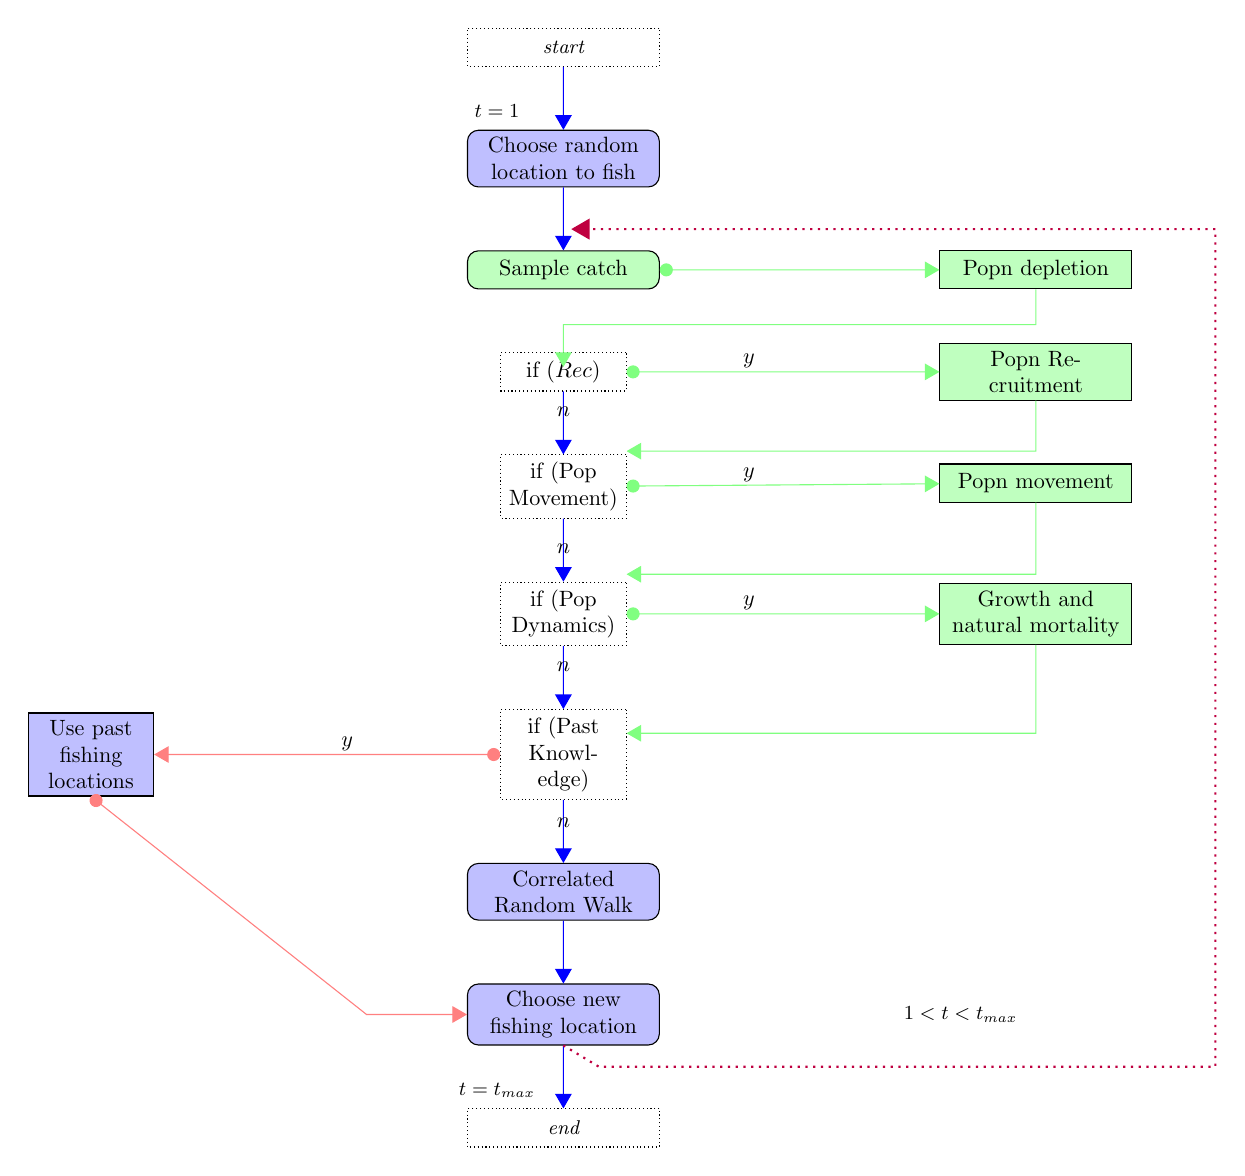
\begin{tikzpicture}[%
    >=triangle 60,              % Nice arrows; your taste may be different
    start chain=going below,    % General flow is top-to-bottom
    node distance=8mm and 60mm, % Global setup of box spacing
    every join/.style={norm},   % Default linetype for connecting boxes
    scale=0.9,
    every node/.style={scale=0.8}]                 
    \label{fig:model}
    % ------------------------------------------------- 
% A few box styles 
% <on chain> *and* <on grid> reduce the need for manual relative
% positioning of nodes
\tikzset{
  base/.style={draw, on chain, on grid, align=center, minimum height=4ex},
  proc/.style={base, rectangle, text width=8em},
  test/.style={base, rectangle, text width=5em},
  term/.style={proc, rounded corners},
  % coord node style is used for placing corners of connecting lines
  coord/.style={coordinate, on chain, on grid, node distance=6mm and 25mm},
  % nmark node style is used for coordinate debugging marks
  nmark/.style={draw, cyan, circle, font={\sffamily\bfseries}},
  % -------------------------------------------------
  % Connector line styles for different parts of the diagram
  norm/.style={->, draw, lcnorm},
  free/.style={->, draw, lcfree},
  cong/.style={->, draw, lccong},
  it/.style={font={\small\itshape}}
}
% -------------------------------------------------
% Start by placing the nodes in the middle
\node [proc, densely dotted, it] (p0) {start};
% Use join to connect a node to the previous one 
\node [term, join, fill=lcnorm!25]      {Choose random location to fish};
\node [term, join, fill=lcfree!25] (p1){Sample catch};
\node [test, densely dotted] (t1) {if $(Rec)$};
\node [test, join, densely dotted] (t2) {if (Pop Movement)};
\node [test, join, densely dotted] (wk) {if (Pop Dynamics)};
\node [test, join, densely dotted] (t3) {if (Past Knowledge)};
\node [term, join, fill=lcnorm!25]  (p2) {Correlated Random Walk};
\node [term, join, fill=lcnorm!25]  (p3) {Choose new fishing location};
\node [proc, densely dotted, join, it] (p7) {end};

% Right nodes
\node [proc, fill=lcfree!25, right=of p1] (p4) {Popn depletion};
\node [proc, fill=lcfree!25, right=of t1] (p5) {Popn Recruitment};
\node [proc, fill=lcfree!25] (p6) {Popn movement};
\node [proc, fill=lcfree!25, right=of wk] (wk1) {Growth and natural
	mortality};

% left nodes
\node [test, fill=lcnorm!25, left=of t3] (t4) {Use past fishing locations};

% -------------------------------------------------
% A couple of boxes have annotations
\node [below=of p0, it, yshift=1.5em,xshift=-3em] {$t=1$};
\node [right=30mm of p3, it] {$1 < t < t_{max}$};
\node [below=of p3, it,xshift=-3em, yshift=1.5em] {$t = t_{max}$};

% -------------------------------------------------
% First, the straight north-south connections. In each case, we first
% draw a path with a (consistently positioned) annotation node, then
% we draw the arrow itself.
  \draw [*->,lcfree!50] (p1) -- (p4);
\path (t1) to node [near start, xshift=2em, yshift=0.5em] {$y$} (p5); 
  \draw [*->,lcfree!50] (t1) -- (p5);
\path (t2) to node [near start, xshift=2em, yshift=0.5em] {$y$} (p6); 
  \draw [*->,lcfree!50] (t2) -- (p6);
\path (t3) to node [near start, xshift=-3em, yshift=0.5em] {$y$} (t4); 
  \draw [*->,lccong!50] (t3) -- (t4);
\path (wk) to node [near start, xshift=2em, yshift=0.5em] {$y$} (wk1); 
  \draw [*->,lcfree!50] (wk) -- (wk1);

% left to right paths
\path (t1) to node [near start, yshift=-0.2em] {$n$} (t2) ;  
\path (t2) to node [near start, yshift=0.8em] {$n$} (t3) ;  
\path (wk) to node [near start, yshift=-0.2em] {$n$} (t3) ;  
\path (t3) to node [near start, yshift=-0.3em] {$n$} (p2) ;  

% ------------------------------------------------- 
% the twisty connectors. Again, we place the annotation
% first, then draw the connector

\node [coord, left=of p3] (c1)  {};  
\draw [*->,lccong!50] (t4.south) -- (c1) |- (p3);

\node[coord, below=of p4] (c2) {};
\node[coord, above=of t1] (c3) {};
\draw [-<,lcfree!50] (p4.south) -- (c2) |- (c3) |- (t1.north);

\node[coord, below=of p5] (c4) {};
\draw [->,lcfree!50] (p5.south) -- (c4) |- ($(t2.east) + (0,0.5)$);

\node[coord, below=of p6] (c71) {};
\draw [->,lcfree!50] (p6.south) -- (c71) |- ($(wk.east) + (0,0.56)$);

\node[coord, below=of wk1] (c7) {};
\draw [->,lcfree!50] (wk1.south) -- (c7) |- ($(t3.east) + (0,0.3)$);

% -------------------------------------------------
% A last flourish which breaks all the rules
\draw [->,purple, dotted, thick, shorten >=1mm]
  (p3.south) -- ++(5mm,-3mm)  -- ++(87mm,0mm) 
  |- node [black, near end, yshift=1.75em, it]
    {} ($(p1.north) + (0,0.3)$);
% -------------------------------------------------
\end{tikzpicture}
\caption{Overview Schematic of simulation model. The blue boxes indicate fleet
	dynamics processes, the green boxes population dynamics processes while
	the white boxes are the time steps at which processes occur; $t$ = tow,
	$tmax$ is the total number of tows; (Rec), (Pop Movement), (Pop
	Dynamics) logic gates for recruitment periods, population movement and
	population dynamics for each of the populations, (Past Knowledge) a
	switch whether to use a random (exploratory) or past knowledge
	(exploitation) fishing strategy.}
%%\label{fig:overview}
\end{figure}
%%%%%%%%%%%%%%%%%%%%%%%%%%



\begin{figure}[!ht]
	\includegraphics[width = \linewidth]{Plots/pop_dist}
	\caption{Simulated spatial dynamics - the four populations abundance
		(log+1) at four time steps.
		}
	\label{fig:9}
\end{figure}	


\begin{figure}[!ht]
	\includegraphics[width = \linewidth]{Plots/f_dynamics}
	\caption{Fishing mortality dynamics - the daily fishing mortalities
		showing weekly and seasonal patterns in exploitation.
		Individual years and the light grey lines, the mean of all
		years the thick black line}
	\label{fig:10}
\end{figure}	

\begin{figure}[!ht]
	\includegraphics[width = \linewidth]{Plots/vessel_move_value}
	\caption{movement of a fleet over a single trip reference overlaid on the
		value field (i.e. sum of the population abundance x catchability x value}
	\label{fig:13}
\end{figure}	


\begin{figure}[!ht]
	\includegraphics[width=\linewidth]{../analysis/Data_Aggregation_space_Rev}
	\caption{Data aggregation at different spatial resolutions over a
		ten year period}
	\label{fig:1}
\end{figure}	

\begin{figure}[!ht]
	\includegraphics[width =\linewidth]{../analysis/Data_Aggregation_time_Rev}
	\caption{Data aggregation at different temporal resolutions over a
		ten-year period}
	\label{fig:2}
\end{figure}	


\begin{figure}[!ht]
	\includegraphics[width = \linewidth]{../analysis/F_trendsREV}
	\caption{Comparison of closure scenarios effect on fishing mortality
		trends. Line colour denotes the timescale, while linestyle
		denotes the spatial resolution.}
	\label{fig:3}
\end{figure}

\begin{figure}[!ht]
	\includegraphics[width =\linewidth]{../analysis/f_diff_effectiveness}
	\caption{Comparison of closure scenario effectiveness based on
		different spatial and temporal resolutions.}
	\label{fig:4}
\end{figure}	

\begin{figure}[!ht]
	\centering
	\includegraphics[width =0.5\linewidth]{./Plots/Closure_fishing_locations_yearly}
	\caption{Closure fishing locations based on annual closures with a
		coarse spatial resolution. Closure location can be seen in red
	in relation to a) before the closure fishing locations, b) after the
	closure fishing locations, c) species 3 habitat distribution}
	\label{fig:17}
\end{figure}	

\clearpage

\section*{References}

\bibliography{simulation_framework}

\end{document}
